\begin{exercises}

\exercise 5.0公斤的物体放在地面上,若物体与地面之间的摩擦系
数是0.30,至少要多大的力才能拉动该物?

\exercise 一个5.0吨的空车箱能使车箱底下的弹簧压缩1.0厘米。如
果在载货后弹簧压缩4.0厘米,求货的质量。

\begin{wrapfigure}[6]{r}{11em}
  \centering
  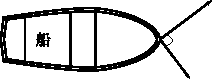
\includegraphics{figure/fig03.22}
  \caption{}
  \label{fig:03.22}
\end{wrapfigure}
\exercise 两人拉纤使船前进,两纤绳互成直角,他们分别用力20公斤和15公
斤(图\ref{fig:03.22}),求使船前进的合力。

\exercise 质量为$ 1.3 \times 10^4 $公斤的火箭
上升时,向上的推力为$ 2.6 \times 10 ^ { 5 } $牛顿,
试求它的加速度。

\exercise 一车的质量为$ 2.85 \times 10 ^ { 5 } $公斤,当车以30公里/小时的速度
行驶时,作紧急刹车。已知制动阻力是车重的0.6倍,求刹车距离
(即刹车后所走的距离)。

\exercise 在电梯中放一磅秤,一个50公斤的人站在磅秤上。求:

(1)当电梯匀速上升或下降时,磅秤指示是多少?

(2)当电梯以4.9米/秒2的加速度上升或下降时,磅秤的指示各为多少?

\exercise 如图\ref{fig:03.23}\,所示,用定滑轮将质量为$ m $的重物送往高处,人
的质量为$ M $,绳不可伸长,绳的质量及它与滑轮的摩擦可忽略。
% 114.jpg
当物体$ m $以匀速上升及以加速度$ a $上升时,人对地面的压力各是多
少?

\begin{figure}[h]
  \begin{minipage}[b]{0.4\linewidth}
    \centering
    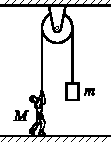
\includegraphics{figure/fig03.23}
    \caption{}
    \label{fig:03.23}
  \end{minipage}
  \begin{minipage}[b]{0.6\linewidth}
    \centering
    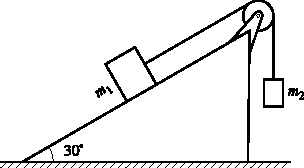
\includegraphics{figure/fig03.24}
    \caption{}
    \label{fig:03.24}
  \end{minipage}
  \vspace{-1.56em}
\end{figure}
\exercise 如图\ref{fig:03.24}\,所示,已知$ m _ { 1 } = 3 . 0 $公斤,$ m _ { 2 } = 2 . 0 $公斤,试求

(1)每一物体的加速度;

(2)~~$ m _ { 2 } $受到的绳子拉力。

\begin{wrapfigure}[8]{r}{13em}
  \centering
  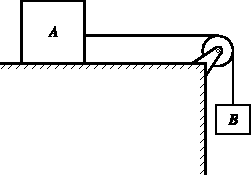
\includegraphics{figure/fig03.25}
  \caption{}
  \label{fig:03.25}
\end{wrapfigure}
\exercise 图\ref{fig:03.25}\,的装置可用来测物体$ A $与桌面间的摩擦系数$ \mu $。设
已知$ A $,$ B $的质量分别是$ m_A $和$ m_B $,它们的加速度是$ a $,试导出
摩擦系数的表达式。

\exercise 两人分别将一小车以同样的加速度推上坡,一人的推力
方向与斜面平行,以$ F_1 $表示;另
一人的推力方向与水平面平行,以$  F_2  $表示。设车与斜面的摩擦系
数$ \mu $及斜面的倾角$ \alpha $已知,求两人推力之比。

\exercise 用起重机吊起一个4吨重的物件,吊索最多可承受5.0吨
的拉力,吊索本身重量可不计,求在下列各情况中吊索所承受的
拉力:

(1)物件吊在空中静止;

(2)物件以25厘米/秒的速度匀速上升;

(3)物件以80厘米/秒的速度匀速下降;
% 115.jpg

(4)物件由静止匀加速上升,在0.5秒内速度增加到20厘米/
秒;

(5)物件由40厘米/秒的速度开始匀加速下降,0.5秒内增加
到80厘米/秒;

(6)要使吊索不断,物体向上的最大加速度是多少?

\begin{wrapfigure}[8]{r}{12.5em}
  \centering
  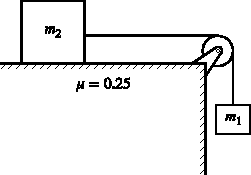
\includegraphics{figure/fig03.26}
  \caption{}
  \label{fig:03.26}
\end{wrapfigure}
\exercise 质量$  m _ { 1 } = 3 0 0  $克的物体
与$  m _ { 2 } = 2 0 0  $克的物体通过定滑轮
用绳连接起来(图\ref{fig:03.26})。物与水
平桌面间摩擦系数$  \mu = 0 . 2 5  $,桌子
不动,绳长不变,绳的质量及绳与滑轮的摩擦可略去。这系统的加
速度是多少?绳的张力是多少?
若互换$ m_1 $与$ m_2 $,有无影响?

\exercise 将质量分别为$ m_1 $, $ m _ { 2 } $ , $m _ { 3 }$ 和$ m $的四个物体连接(图\ref{fig:03.27})
桌面与这些物体之间的摩擦系数都是$ \mu $。设绳长不变,桌子与滑
轮位置不变,绳子的质量及绳与滑轮间的摩擦可忽略不计。求这
系统的加速度以及各物体之间的张力$  T _ { 1 }  $,$  T _ { 2 }  $,$  T _ { 3 }  $。
\begin{figure}[h]
  \centering
  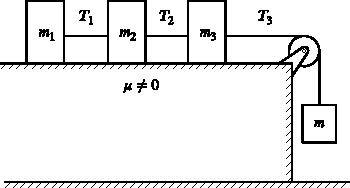
\includegraphics{figure/fig03.27}
  \caption{}
  \label{fig:03.27}
\end{figure}

\exercise 质量分别为$ m_1 $,$  m _ { 2 } $ 和$ m_3 $的三个物体($ m _ { 2 } > m _ { 1 } $),用绳子按
图\ref{fig:03.28}~所示连接。$ A $和$  B  $是两个轻滑轮。设斜面和滑轮位置不变,绳
长不变,略去摩擦力和绳子的质量。求系统的加速度$ a $和绳中的
% 116.jpg
张力$  T _ { 1 }  $,$  T _ { 2 }  $;$ A  $点承受的力;绳$ d $上的张力。

\begin{wrapfigure}[7]{r}{14.5em}
  \centering
  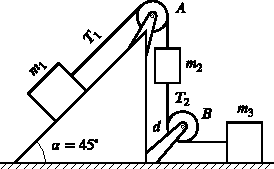
\includegraphics{figure/fig03.28}
  \caption{}
  \label{fig:03.28}
\end{wrapfigure}
\exercise 一个学生要确定一个盒子与一块乎板之间的静
摩擦系数$ \mu _ 0 $及滑动摩擦系数 $\mu$。他把盒子放在平板上,
渐渐抬高板的一端,当板的倾角(即板与水平之夹角)达
\ang{30}时,盒子开始滑动,并
恰好在4.0秒内滑下4.0米距离。试由这些数据确定 $\mu_0$及 $\mu$。

\begin{wrapfigure}[6]{r}{17em}
  \centering
  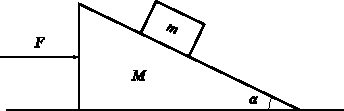
\includegraphics{figure/fig03.29}
  \caption{}
  \label{fig:03.29}
\end{wrapfigure}
\exercise 如图\ref{fig:03.29},质量为$ M $的三角形斜面上放一个小质量物体$ m $,
三角形物体放在水平面上,假设所有接触都是光滑的。求:

(1)必须用多大的水平推力$ F $,才能使$ m $相对于$ M $为静止?

(2)此时系统的加速度$ a $有多大?

\exercise 收尾速度问题。空气对物体的阻力由许多因素决定。然
而,一个有用的近似公式是,阻力$  \vec{f} _ { p } = - \beta \vec{v}  $,其中$\vec{v}$是物体的速度,
$\beta$是一个与速度无关的常数。现在考虑空气中的一个自由下落物
体,将$ Z $轴的正方向取为竖直向下。

(1)给出落体的牛顿方程。

(2)当物体的速度$  v( t _ 0)  $等于多少时,物体不再加速(这个速
度叫做收尾速度)?

(3)试证,速度随时间变化的关系为:
\begin{equation*}
  v ( t ) = v ( t _ 0 ) \left( 1 - \e ^ { - \frac { \beta } { m } t } \right)
\end{equation*}
并作出$ v \mathdash t $曲线。

% 117.jpg
(4)定性地画出这种运动的$ z \mathdash t $图及$ a \mathdash t $图。

\exercise 升降机中固定着一个倾角为$ \theta $的光滑斜面,一小物体沿着
斜面下。在以下几种情况下,求物体相对于斜面的加速度。

(1)升降机以恒定速率$ v $下降;

(2)升降机以恒定速率$ v $上升;

(3)升降机以加速度$ a $下降;

(4)升降机以减速度$ a $下降;

(5)升降机的吊缆拉断;

(6)在情况(3)中,斜面与物体间的作用力多大?

\exercise 质量分别为$ M $和$  M + m  $的两个人,分别拉住定滑轮两边
的绳子往上爬(图\ref{fig:03.30})。开始时两人与滑轮的距离都是$ h $。设滑轮
和绳子的质量以及定滑轮轴承处的摩擦力均可不计,绳长不变。
试证明,如果质量轻的人在$ t $秒种爬到滑轮,这时质量重的人与
滑轮的距离为
\begin{equation*}
  \frac { m } { M + m } \left( h + \frac { 1 } { 2 } g t ^ { 2 } \right)
\end{equation*}

\begin{figure}[h]
  \begin{minipage}[b]{0.4\linewidth}
    \centering
    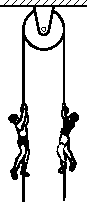
\includegraphics{figure/fig03.30}
    \caption{}
    \label{fig:03.30}
  \end{minipage}
  \begin{minipage}[b]{0.6\linewidth}
    \centering
    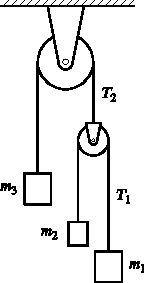
\includegraphics{figure/fig03.31}
    \caption{}
    \label{fig:03.31}
  \end{minipage}
  \vspace{-1.56em}
\end{figure}
\exercise 一动滑轮与一定滑轮连接(图\ref{fig:03.31}) ,已知$  m _ { 1 } = 4 0 0  $克,$  m _ { 2 } = 2 0 0  $克,$  m _ { 3 } = 4 0 0  $克,略去摩擦及动滑轮的质量,设绳长不变,绳
的质量可不计。求每个物体的加速度及各绳中的张力。

\begin{wrapfigure}[4]{r}{16em}
  \centering
  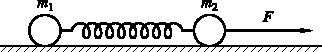
\includegraphics{figure/fig03.32}
  \caption{}
  \label{fig:03.32}
\end{wrapfigure}
\exercise 质量为$  m _ { 1 } = 1 0  $公斤和$  m _ { 2 } = 2 0  $公斤的
两物体,用轻弹簧连接在一起水平放在光滑桌
面上,以$  F = 2 0 0  $牛顿的力沿弹簧方向作用于$  m _ { 2 }  $,使$  m _ { 1 }  $得到加速
度$  a _ { 1 } = 1 2 0 $厘米/秒\textsuperscript{2},$  m _ { 2 }  $的加速度$  a _ { 2 }  $应是多少?

\exercise 假使汽车能以速率$  v = 1 0 0  $公里/小时驶过半径$  R = 2 0 0  $
米的水平弯道,车胎与地面间的摩擦系数至少要多大?

\begin{wrapfigure}[10]{r}{9em}
  \centering
  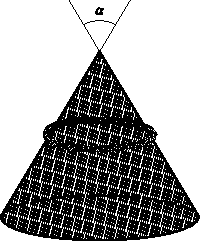
\includegraphics{figure/fig03.33}
  \caption{}
  \label{fig:03.33}
\end{wrapfigure}
\exercise 如图\ref{fig:03.33}所示,一长为$ L $、质量为
$ M $的均匀链条,套在一表面光滑、顶角为$ \alpha $
的圆锥上。当链条在圆锥面上静止时,链
条中的张力是多少?

\exercise 长为$  l = 4 0  $厘米的绳,一端固定于
一点$ O $,另一端系一质量$  m = 1 0 0  $克的小球,
绳不可伸长,其质量可忽略。让小球在铅
直平面作圆周运动。问:

(1)小球通过最高点时,若绳的张力为零,小球的速度$  v _ { 0 }  $为多少?

(2)若小球通过最高点时的速度为$  2 v _ { 0 }  $,绳中的张力$ T $是多少?

\exercise 如图\ref{fig:03.34}~所示,一细绳穿过光滑的、不动的细管,两端分
别拴着质量为$ m $和$ M $的小球。当小球$ m $绕管子的几何轴转动时,$ m $
到管口的绳长为$ l $,与竖直的细管夹角为$ \theta $。细管半径可以忽略,
求小球的速度和它所受的向心力;并证明:$  \cos \theta = \dfrac { m } { M }  $; 以及小球
的转动周期
$ T = 2 \uppi \sqrt{\dfrac { l m } { M g }}  $。

% 119.jpg
\begin{wrapfigure}[10]{r}{9.5em}
  \centering
  
\includegraphics{figure/fig03.34}
  \caption{}
  \label{fig:03.34}
\end{wrapfigure}
\exercise 一个质量为$ m $的小物体放在碗内,设碗的内表面是球形的光滑面。当碗
以匀角速度绕通过球心的竖直轴转动时,$ A $在什么高度才有可能紧贴碗壁随碗
一起转动?若一开始$ A $在碗底又将怎样?

\exercise 顶角为$ \theta $的圆锥形漏斗垂直于水平面放置(图\ref{fig:03.35}),漏斗内有一质量为$ m $
的小物体,$ m $距漏斗底的高度为$ h $。问:

(1)如果$ m $与锥面间无摩擦,要使$ m $停留在$ h $高度随锥面一起绕其几何轴以匀角
速度转动,$ m $的速率应是多少?

\begin{wrapfigure}[8]{r}{9.5em}
  \vspace{-3.12em}
  \centering
  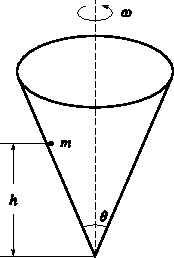
\includegraphics{figure/fig03.35}
  \caption{}
  \label{fig:03.35}
\end{wrapfigure}
(2)如果$ m $与锥面间的摩擦系数为 $\mu$,要使$ m $稳定在高度随锥面一起以匀角速
度转动,但可以有向上或向下运动的趋势,则$m$的速率范围是什么?

\exercise 一汽车驶过一半径为$ R $的水平弯道,路面倾角为$ \theta $(图\ref{fig:03.36}),车轮与路面
间的摩擦系数为$ \mu $。求汽车在弯道上不侧滑的速率范围,若超出此范围,车会怎样?

\begin{figure}[h]
  \centering
  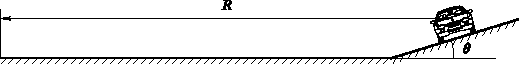
\includegraphics{figure/fig03.36}
  \caption{}
  \label{fig:03.36}
\end{figure}

\exercise 一根重量为$ W $的均匀的绳子,悬结于两根竖直于地面上
的杆之间,绳子两端的高度一样,并分别与杆成$ \theta $角,求

(1)绳子任一端处的张力;

(2)绳子中点的张力。

% 120.jpg
\exercise 把一段单位长度的质量为$ \lambda $的绳子$ AB $挂在平置的光滑圆
木上,$ A $端固定在圆木的最高点,绳长等于该圆木的1/4周长(图\ref{fig:03.37}) ,圆木半径为$ R $。

(1)画出$ \theta $与$ \theta + \Delta \theta$之间这小段绳子的受力图,求出绳中张力
$ T (\theta) $的表达式;并证明,绳子上端的张力为$  T _ { A } = \lambda R g  $;

(2)写出圆木作用在$ \theta $与$  \theta + \Delta \theta  $之间小段绳子上的法向力$ N $
的表达式。对这个力的水平分量求积分(对整段绳子),并说明结果的物理意义。
\begin{figure}[h]
  \begin{minipage}[b]{0.5\linewidth}
    \centering
    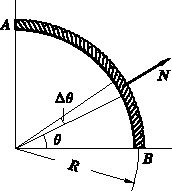
\includegraphics{figure/fig03.37}
    \caption{}
    \label{fig:03.37}
  \end{minipage}
  \begin{minipage}[b]{0.5\linewidth}
    \centering
    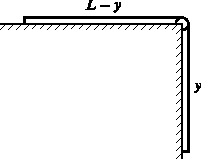
\includegraphics{figure/fig03.38}
    \caption{}
    \label{fig:03.38}
  \end{minipage}
  \vspace{-1.56em}
\end{figure}

\exercise 一长为$ L $,质量为$ M $的均匀电缆,静止放在光滑的桌面
上,一端伸出桌的边沿(图\ref{fig:03.38}),在桌边沿处有一可忽略摩擦的小
滑轮,因此,滑轮两边的张力恰好相等。根据定义,电缆两自由
端的张力为零。

(1)当长为$ y $的一段伸出桌的边沿时,电缆的加速度$ a $是多少?

(2)假使长度为$  y _ { 0 }  $的一段电缆伸出桌的边沿时,放手让电缆
由静止开始自由运动,给出$ y(t) $。

\exercise 一周长为$ l $,质量为$ M $的圆环,绕圆心以匀角速度$ \omega $在水
平面内转动,求圆环上的张力$ T $。

\exercise 一质量为$ m $的小物体,由两根长为$ l $的细绳拴在一竖直的
转轴上(图\ref{fig:03.39})当轴和物体都以匀角速度$ \omega $转动时,两根绳子
与轴都成\,\ang{45}\,角。
% 121.jpg

(1)画出物体的受力图;

(2)分别求出两根绳子中的张力$ T_1 $及$ T_2 $。

\begin{figure}[h]
  \begin{minipage}[b]{0.5\linewidth}
    \centering
    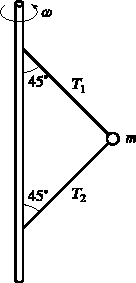
\includegraphics{figure/fig03.39}
    \caption{}
    \label{fig:03.39}
  \end{minipage}
  \begin{minipage}[b]{0.5\linewidth}
    \centering
    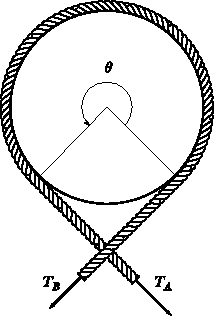
\includegraphics{figure/fig03.40}
    \caption{}
    \label{fig:03.40}
  \end{minipage}
  \vspace{-1.56em}
\end{figure}

\exercise 一种在船上使用的称为绞盘的装置,用来控制在巨大张
力作用下的绳。绳索绕在绞行的固定圆柱上,通常绕若干匝(图
\ref{fig:03.40})。绳子一端承受巨大的拉力$  T _ { B }  $,而海员却可以小得多的力
$ T_A $拽住绳子的另一端。设绳子与圆柱表面的摩擦系数为$ \mu $,绳子
绕圆柱的角度为$ \theta $,求绞盘不动时$ T_A / T_B $。

\lbr 提示:参见例题6的结果,对$ \theta $进行积分。\rbr

\exercise 一质量为$ M $的斜面静止在粗糙的地板上(图\ref{fig:03.41})。斜面
上端有一光滑而轻的小滑轮,一绳跨过滑轮吊住一质量为$ m_1 $的物
体,绳的另一端拴住质量为$ m_2 $的物体,$ m _ { 2 } $在斜面上无摩擦地滑动,
斜面与地板夹角为$ \theta $,试求:

(1)\;$ M $,$ m _ { 1 } $,$  m _ { 2 }  $各物体所受的力;

(2)假定斜面静止,写出系统的牛顿方程,并求$ m_1 $,$ m_2 $的加
速度及绳中之张力;

(3)若要斜面保持静止,斜面与水平面间的摩擦系数至少要
% 122.jpg
多少?

\begin{figure}[h]
  \centering
  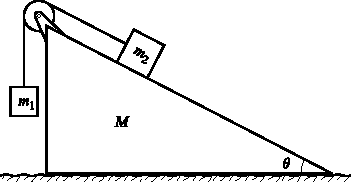
\includegraphics{figure/fig03.41}
  \caption{}
  \label{fig:03.41}
  \vspace{-0.5em}
\end{figure}

\exercise 一小木块放在倾角为$ \theta $的斜面上(图\ref{fig:03.42}),木块与斜面间
的静摩擦系数为$ \mu $。设$  \tg \theta > \mu $。若给斜面一个水平加速度$ a $,又要
木块在斜面上保持相对静止,求$ a $的可能范围。
\begin{figure}[h]
  \centering
  
\includegraphics{figure/fig03.42}
  \caption{}
  \label{fig:03.42}
  \vspace{-0.5em}
\end{figure}

\exercise 一车以速率$ v $通过半径为$ R $的圆形拱桥(图\ref{fig:03.43})。汽车质
量为$ m $,不计摩擦,桥所受到的压力是多少?如果桥是凹形的又
怎样?
\begin{figure}[h]
  \centering
  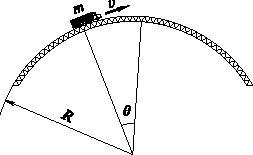
\includegraphics{figure/fig03.43}
  \caption{}
  \label{fig:03.43}
\end{figure}
\end{exercises}